\begin{figure*}[tbp]
\newcommand{\figheight}{0.33\textwidth}
\newcommand{\figwidth}{0.485\textwidth}
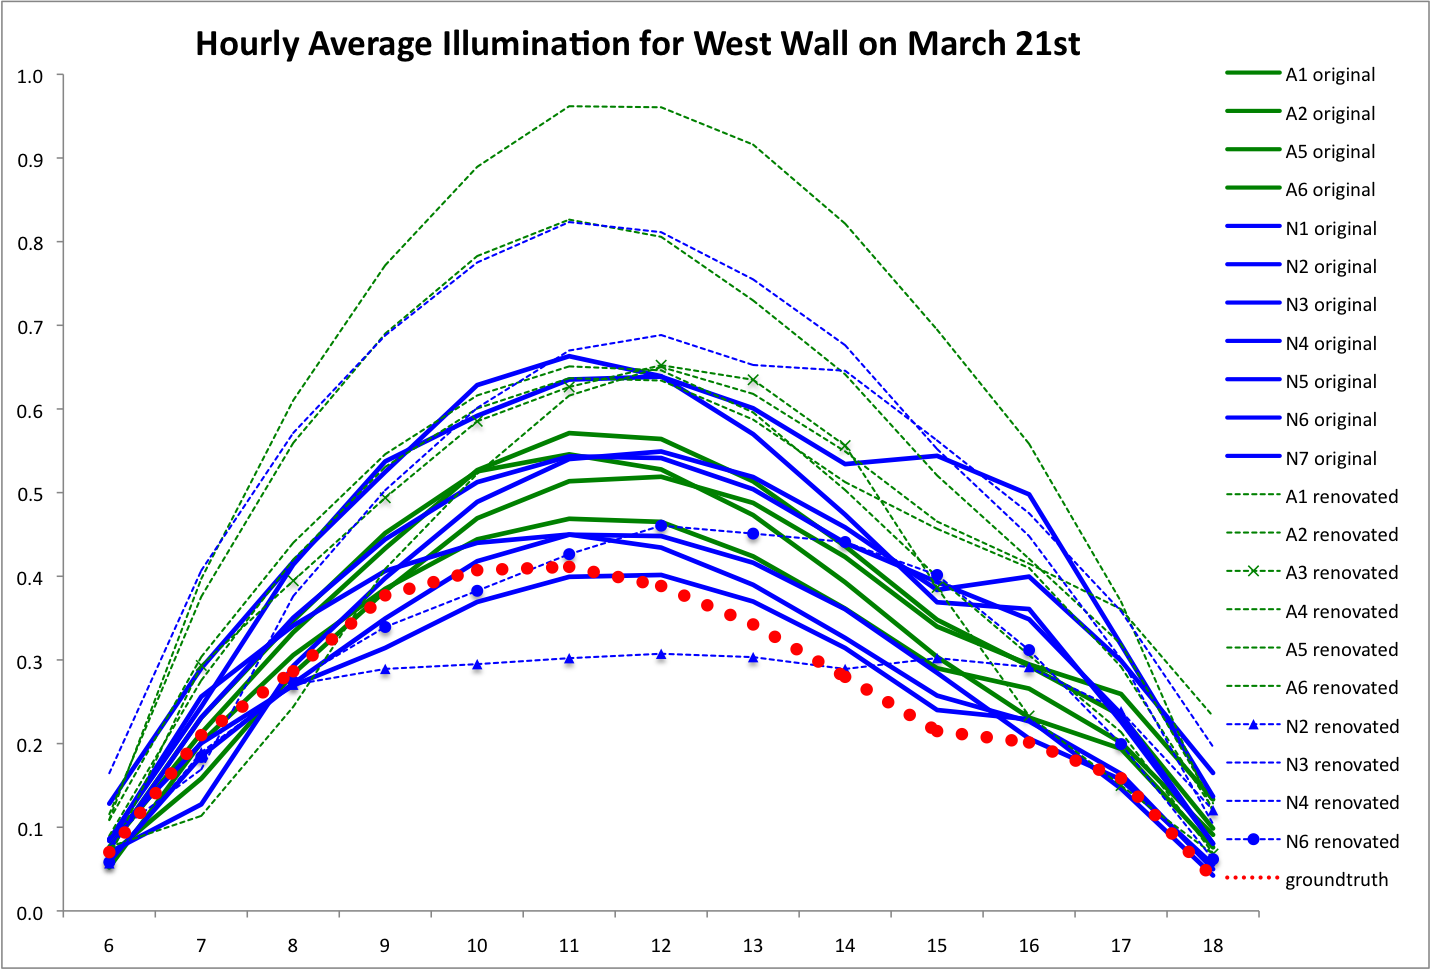
\includegraphics[height=\figheight,width=\figwidth]{hourly_west_march_21.png}\hfill
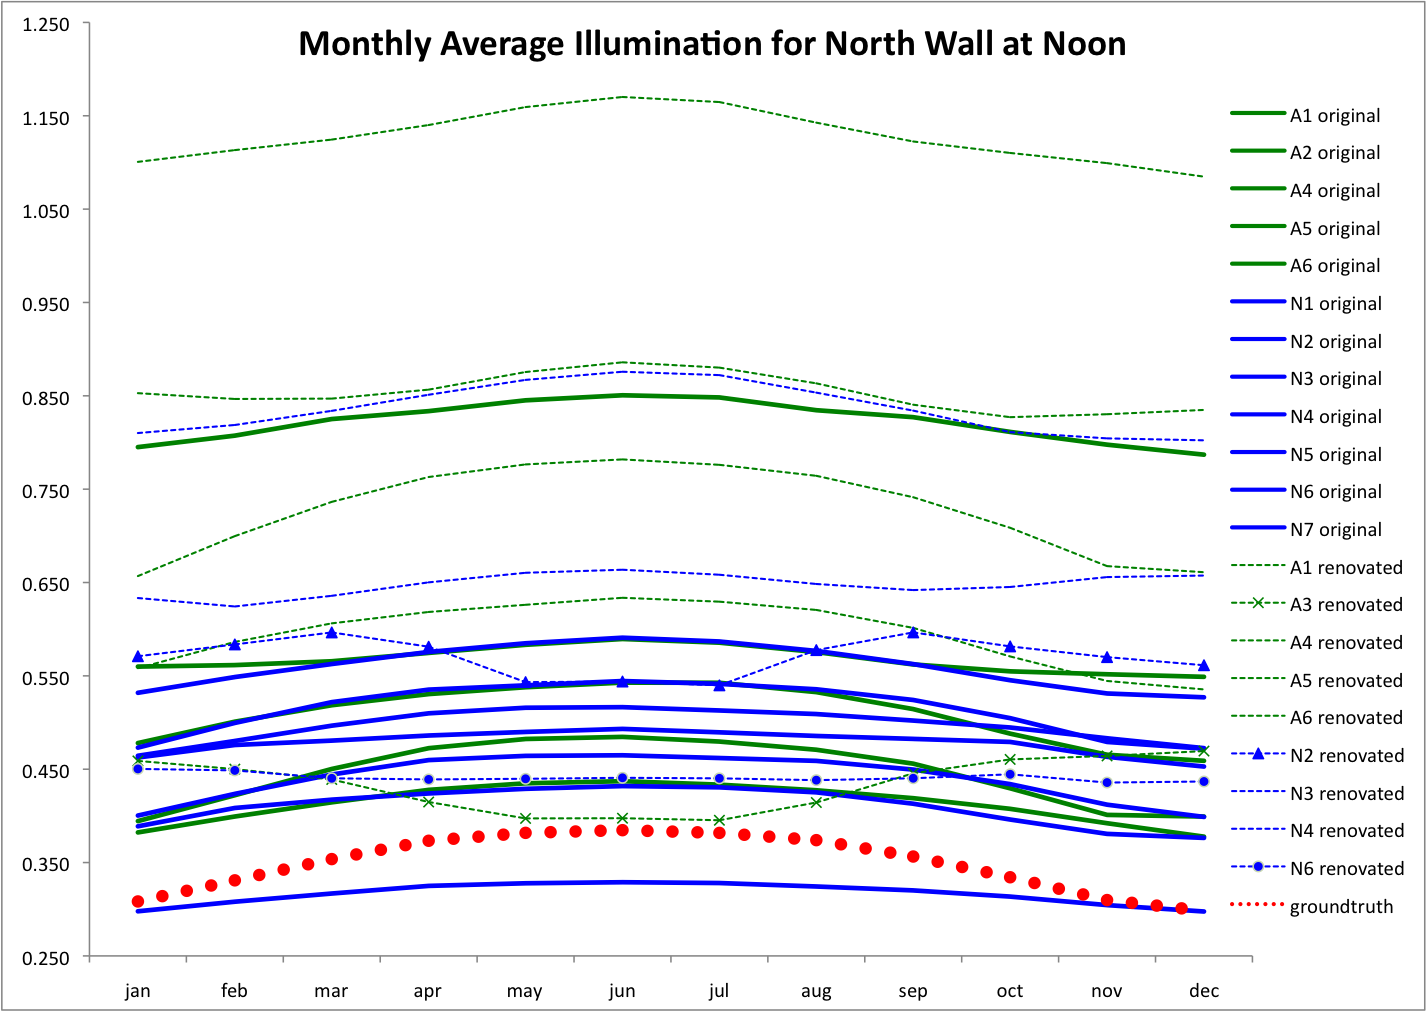
\includegraphics[height=\figheight,width=\figwidth]{montly_average_north_wall_noon.png}\vspace{0.1in}\\
\begin{minipage}{2in}~\end{minipage} \hfill 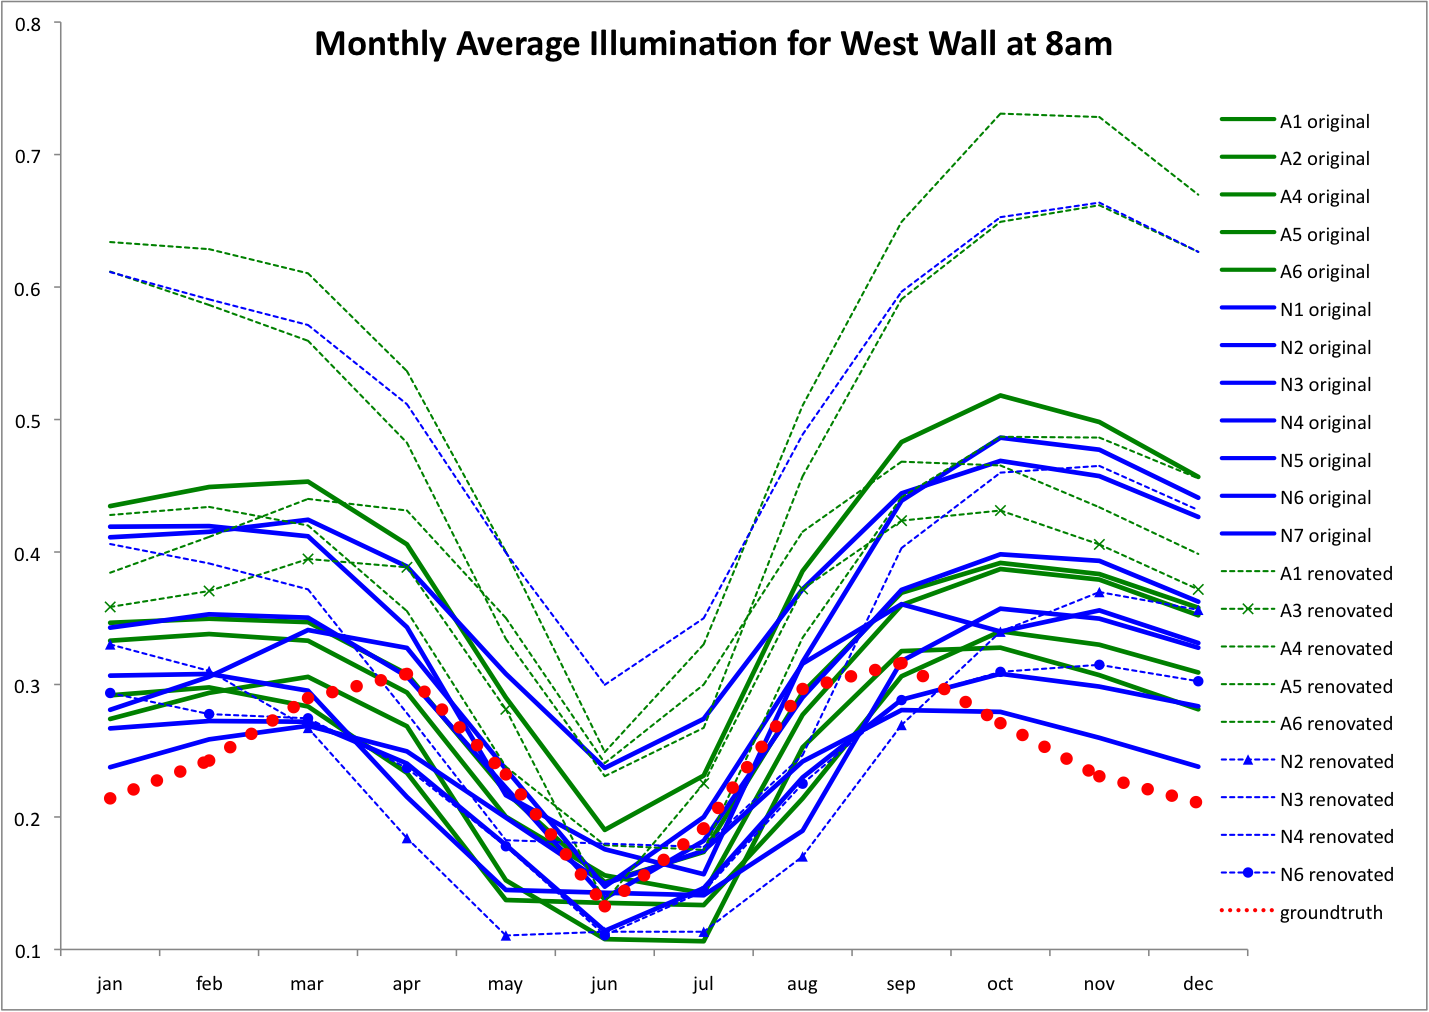
\includegraphics[height=\figheight,width=\figwidth]{monthly_average_west_wall_8am.png}\vspace{-0.2\textwidth}\\
\vspace{-0.7in}
\caption{
%
Plots analyzing the daily and \protect\\
seasonal variations in illumination for the \protect\\ 
users original and renovated models.  We \protect\\ 
observe that on average the models built by \protect\\
 participants resulted in a significant \protect\\
over-estimate of the available daylighting.  \protect\\
In the top right plot,  we can clearly identify \protect\\
the 3 users who focused on renovations to \protect\\
reduce glare (A3, N2, and N6).
%
\label{figure:plots}
}
\vspace{0.1in}
\end{figure*}
